\chapter{System Design}

The goal of this project is to develop a model for cloud detection based on U-Net architecture employing semantic segmentation.

\section{Dataset Design}

The model is trained using Landsat 8 satellite images. L8 dataset contains 38 scenes with each scene divided into 384*384 pixels.There were 8,400 patches created for training and 9,200 patches were created for testing. Each patch consist of four spectral channels which are Red, Green, Blue and Near Infrared. It is important to note that channels are not combined in the dataset. 

The patches were examined to evaluate the presence of a significant number of geographical challenges within the dataset for the model's evaluation. Patches from various channels were combined into a single patch and thoroughly reviewed to achieve this. Following that, it was determined that the dataset is appropriate for training the model.

All of the channelized images were combined and processed to create a dataset that is model-compatible.  This dataset is stored in a location called "hub". This storage technique makes it simple for any Python environment to use the dataset.

The dataset includes unchallenging and challenging images for training and testing of the model. Examples of unchallenging images are given below Figure \ref{easy} while challenging images are provided below Figure \ref{hard}. 

\begin{figure}[htp]
    \centering
    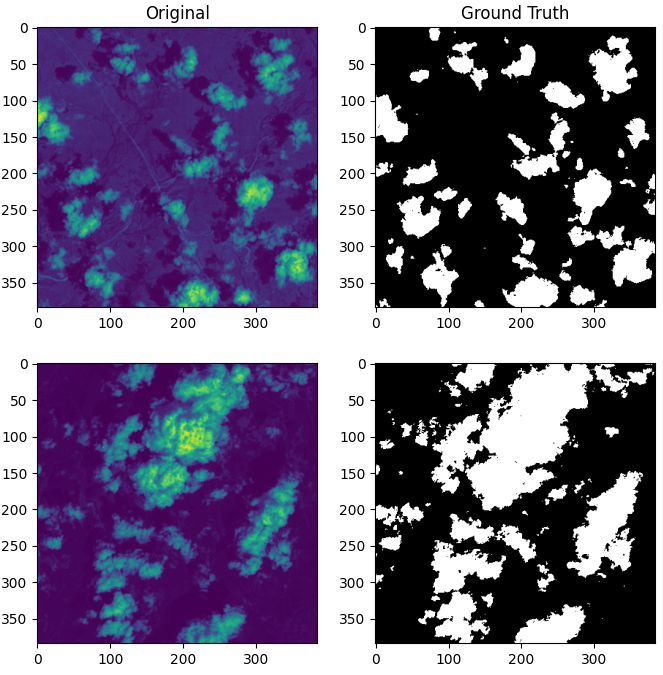
\includegraphics[width=10cm]{projectChapters/images/easy.png}
    \caption{Example for unchallenging train images}
    \label{easy}
\end{figure}

\begin{figure}[htp]
    \centering
    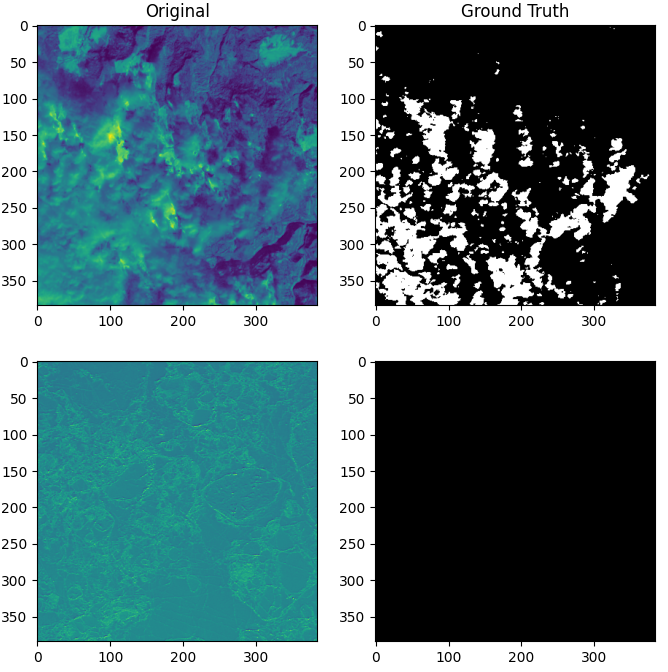
\includegraphics[width=10cm]{projectChapters/images/hard.png}
    \caption{Example for challenging train images}
    \label{hard}
\end{figure}
\newpage
\section{Cloud Detection Algorithm}

Deep learning is a machine learning subject which is focused on training artificial neural networks how to recognize information and make predictions or choices. The algorithms develop to identify patterns and extract relevant information from massive volumes of data. They are intended to learn layered structures for input data by gradually learning increasingly complicated and abstract attributes. These hierarchical representations are learned through an approach known as training, in which the neural network's internal parameters are adjusted based on the input data and the desired output.The artificial neural network, which consists of numerous layers of linked nodes, is the most significant component of deep learning. Each node in the network conducts a basic computation and sends the results to the other nodes in the network. Weights are related to node connections, which are modified during the training phase to optimize the network's performance.

Project is created with a U-Net-based software implementation of a Convolutional Neural Network for image segmentation. A deep learning architecture known for its excellent results in image segmentation tasks is U-Net. Effective feature extraction and spatial information reconstruction are made possible by the system's distinctive U-shaped structure, which includes an encoding and decoding network.

The Encoder Network is similar to convolutional neural network. It employs convolutional and pooling layers to extract high-level features and capture context from input images, therefore reducing the spatial dimensions and increasing the number of feature channels. The Decoder Network; employs upsampling, concatenation operations, and convolutional layers to improve spatial resolution and produce a segmentation map. It combines feature maps and improves spatial resolution to provide the decoder precise localization data. With the use of skip connections, the respective levels of the encoder and decoder are connected by U-Net.

The final layer of the U-Net architecture is a 1x1 convolutional layer followed by a softmax activation function. The result is a pixel-by-pixel prediction probability map, where each pixel denotes the likelihood that a certain class is present. 
\newpage
The represantation of the U-NET Architecture is given below Figure \ref{unet}.
\begin{figure}[htp]
    \centering
    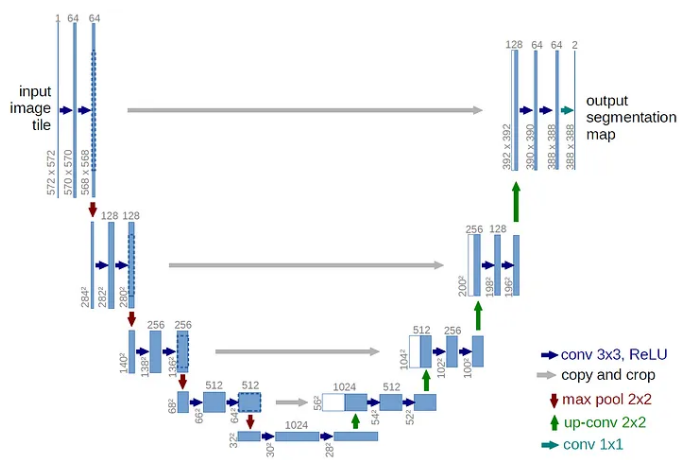
\includegraphics[width=10cm]{projectChapters/images/unet.png}
    \caption{U-NET Architecture}
    \label{unet}
\end{figure}

The model is created using a collection of cloud pictures and ground truth masks supplied by the hub library. The code offers features for data loading and preprocessing, model definition and training, likewise performance evaluation on a test set. The Adam optimizer and the binary cross-entropy loss function are used to optimize the model. Evaluation metrics such as precision, recall, accuracy and mean Intersection over Union are utilized to assess the model's performance. During the training, checkpoints are implemented to store the optimal weights based on validation performance. Finally, the trained model is applied to forecast segmentation predictions on a test set of images.

The algorithm patterns are represented by the block diagram shown in Figure \ref{block}.

\begin{figure}[htp]
    \centering
    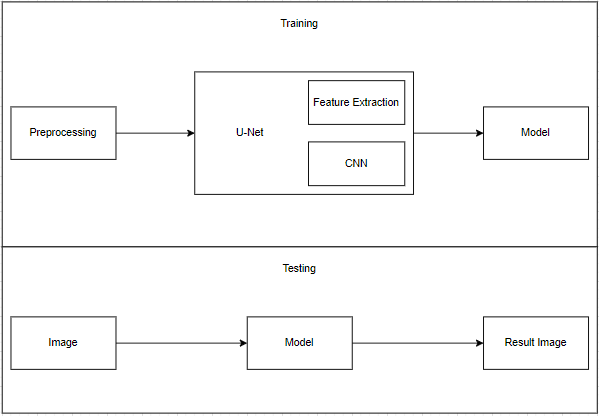
\includegraphics[width=10cm]{projectChapters/images/blok_diyagram.png}
    \caption{Block Diagram}
    \label{block}
\end{figure}
